\documentclass[17pt,a4paper,landscape]{extarticle}
\usepackage[margin=2.35cm,top=0.12cm,left=1.05cm]{geometry}
\usepackage{amsmath}
\usepackage{amssymb}
\usepackage{tasks}
\usepackage{tikz}
\usepackage{xcolor}
\usepackage[sfdefault,lf]{FiraSans}
\renewcommand{\familydefault}{\sfdefault}
\setlength{\parindent}{0pt}
\pagestyle{empty}
\settasks{label=\textbf{\arabic*.}, label-width=2.2em, item-indent=2.95em, column-sep=2.1cm, after-item-skip=5.1em}
\renewcommand{\arraystretch}{1.15}
\everymath{\displaystyle}

\newcommand{\twocointree}{%
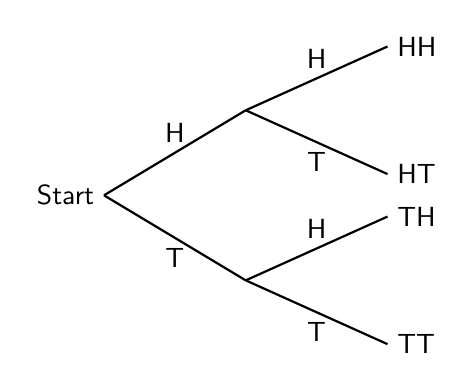
\begin{tikzpicture}[x=0.9cm,y=0.9cm]
  \draw[thick] (0,0) -- (2,1.2) node[midway,above] {H};
  \draw[thick] (0,0) -- (2,-1.2) node[midway,below] {T};
  \draw[thick] (2,1.2) -- (4,2.1) node[midway,above] {H};
  \draw[thick] (2,1.2) -- (4,0.3) node[midway,below] {T};
  \draw[thick] (2,-1.2) -- (4,-0.3) node[midway,above] {H};
  \draw[thick] (2,-1.2) -- (4,-2.1) node[midway,below] {T};
  \node[left] at (0,0) {Start};
  \node[right] at (4,2.1) {HH};
  \node[right] at (4,0.3) {HT};
  \node[right] at (4,-0.3) {TH};
  \node[right] at (4,-2.1) {TT};
\end{tikzpicture}%
}


\begin{document}
\sffamily
\boldmath

\vspace*{0.4em}
{\LARGE \textbf{Proficient}}
\begin{tasks}(2)
\task {Use this tree to list the sample space for tossing two coins.

\vspace{0.4em}
\twocointree}
\task {Use the tree to say how many outcomes are in the sample space.

\vspace{0.4em}
\twocointree}
\task {Use the tree to write the probability of getting exactly one head.

\vspace{0.4em}
\twocointree}
\task {Use the tree to write the probability of getting two tails.

\vspace{0.4em}
\twocointree}
\task {A fair die is rolled. What is the probability of getting a factor of $6$?}
\task {A fair die is rolled. What is the probability of getting a multiple of $3$?}
\task {A spinner has $5$ equal sectors labelled $1,2,3,4,5$. What is the probability of landing on a prime number?}
\task {A bag has $8$ counters: $3$ red, $2$ blue, and $3$ green. What is the probability of picking a blue counter?}
\task {A standard deck card is chosen. What is the probability that the card is a heart?}
\task {A standard deck card is chosen. What is the probability that the card is black?}
\task {Which is more likely: rolling a number greater than $4$ on a die or picking a blue counter from a bag with $1$ blue and $3$ red counters?}
\task {Which is more likely: drawing a heart from a deck or getting heads on a fair coin?}
\end{tasks}

\end{document}
